% $  Id: validation.tex  $
% !TEX root = main.tex


%%
\section{Validation}
\label{sec:validation}

This section provides empirical experimentation of the \ac{ML} techniques introduced in the previous 
section. Two application for pattern recognition were selected to execute each of the techniques. The 
first application uses existing housing system data to learn and predict market prices. The second 
application, uses pattern recognition for the identification of objects (flowers) in an image.

%%%%
\subsection{Execution Environment}

The first experiment used data provided by Google's Machine Learning Crash 
course~\cite{mlchrome18}. The experiment was run using TensorFlow directly on the Google 
Chrome browser using google's collaboration platform. 
%Nonetheless, it is possible to execute the program offline which requires the user to set up a local Datalab environment by installing Docker~\cite{docker18}.   
The second experiment was developed using TensorFlow version 1.0 running in a Jupiter 
Notebook with python 3 accessed through Anaconda. 
Both experiments were run on a 2013 Intel Core i5 MacBook Air with macOS Sierra version 10.12.6.

%%%%
\subsection{Learning with Linear Regression}

For the first experiment resources and learning material were taken from Google’s Artificial 
Intelligence course. The course provides knowledge for beginners and experts, as well as practice 
material and online classes. The experiments uses data from 1990’s housing system in California. 
Based on this data, we want to build a model capable of predicting median house value at the 
granularity of city blocks based on a specific feature from the available data set (\eg median house age, 
median value)~\cite{mlchrome18}. 

When starting a \ac{ML} project, the most important part is to understand the available data.
Taking advantage from data insights it is possible to obtain a more accurate model. The housing data 
(\ie \emph{data frame}) used in this experiment is composed of nine features,\footnote{\url{https://storage.googleapis.com/mledu-datasets/california_housing_train.csv}} namely: 
\begin{enumerate*}[label=(\arabic*)]
\item \tensorcode{longitude},
\item \tensorcode{latitude},
\item median age (\tensorcode{housing_median_age}),	
\item total number of rooms (\tensorcode{total_rooms}),	
\item total number of bedrooms (\tensorcode{total_bedrooms}),
\item \tensorcode{population},	
\item \tensorcode{households},
\item median income (\tensorcode{median_income}), and
\item	median house value (\tensorcode{median_house_value}).
\end{enumerate*}
These features are classified according to their data type --that is, categorical (\eg text), or numeric 
(\eg number, integer, float). Features describe how the model should use raw input data from a 
features dictionary. Raw data, in TensorFlow, is processed through \emph{Estimators}, exposed as 
the high-level API of the language~\cite{tensor18}. \fref{lst:feature-configuration} shows the definition 
of a desired input feature, and its classification as a numeric feature, using the TensorFlow high-level 
API.

\begin{tensorflow}[
	label={lst:feature-configuration},
	caption={Feature definition and classification}]
 # input feature is designated
 my_feature = california_housing_dataframe[["total_rooms"]]

 # A numeric feature column for total_rooms is configured.
 feature_columns = [tf.feature_column.numeric_column("total_rooms")]
\end{tensorflow}

The goal for this experiment is to estimate the median house value based on historic data, available to 
users. These characteristics suggest to use the linear regression model for the estimation.
As explained in \fref{sec:linear-regression}, we create the linear regression model 
(\fref{ln:linear-model}) based on the gradient  decent (Lines \ref{ln:gradient-init}-\ref{ln:gradient-end}) as 
shown in \fref{lst:lrm}.

\begin{tensorflow}[numbers=left,
	label={lst:lrm},
	caption={Generation of the linear regression model}]
 #Gradient Descent declaration
 my_optimizer=tf.train.GradientDescentOptimizer(learning_rate=0.0000001) ` \label{ln:gradient-init} `
 my_optimizer = tf.contrib.estimator.clip_gradients_by_norm(my_optimizer, 5.0) 
 ` \label{ln:gradient-end} `

 #Include the feature columns and optimizer in the configuration of the  linear regression model.
 #Learning rate is set to  0.0000001 for the Gradient Descent
 linear_regressor = tf.estimator.LinearRegressor(feature_columns=feature_columns, optimizer=my_optimizer) ` \label{ln:linear-model} `
\end{tensorflow}

As with other \ac{ML} techniques, in order to make a prediction, the model needs to be trained using 
available data. In order to train the model, it is necessary to \emph{batch}, \emph{preprocess}, and 
\emph{shuffle} the data.  This is to assure that the model will not be trained on biased data. 
Training a linear regression model requires a function (\tensorcode{input_fn} in 
\fref{lst:training}) characterized by the feature to make the prediction (\tensorcode{my_feature}), as 
well as the targets (of the estimation). Finally developers are required to define the number of steps 
in which the model will be trained.

\fref{lst:training} shows the training definition for the the housing system data. in this example we 
train the model for 100 steps, using as input feature \tensorcode{total_rooms}, defined in 
\fref{lst:feature-configuration}. 

\begin{tensorflow}[
	label={lst:training},
	caption={Model training}]
 _ = linear_regressor.train(
    input_fn = lambda:my_input_fn(my_feature, targets),
    steps=100
 )
\end{tensorflow}

The decision of using 100 training steps is the outcome of the model fitting process, where developers 
are required to fine tune the model parameters to assure accurate predictions. During training, it is 
required to measure the effectiveness of the model. If prediction errors are identified, for example 
using the least square error, it is required to adjust the model \emph{hyperparameters}. That is, 
modifying the batch size, learning rate, or number of steps, to find a good fit with low prediction error. 
Normally, hyperparameters will change from project to project.

During the fitness process, the model should be fit to foster \emph{generalization}. 
Generalization refers to the model’s ability to adapt to new, previously unseen data, drawn from the 
same distribution as the one used to create the model.  Generalization allows for all training examples 
to be correctly classified. If the model works well with predictions on the test set and the data set, then 
this is a good indicator about how the model is going to perform when dealing with new unseen data.  


%%%%
\subsection{Learning with \acl{NN}}

For the second experiment we developed a pattern recognition \ac{ML} algorithm. in particular the 
goal of this project is to accurately classify flowers detected on an image, based on a dataset of 
plant measurements, such as: sepal length, sepal width, petal length and petal width. Specifically, 
the model should classify flowers into one of three Iris flowers: Iris Setosa, Iris Versicolor and Iris 
Virginica. This experiment is developed using a \ac{NN}, using the content provided in TensorFlow's 
website~\cite{tensor18}. 
 
Similar to the linear regression model, in order to use \ac{NN} in pattern recognition, it is necessary 
to provide a representation of the the entities to recognize as a data frame. \fref{fig:object-rep} shows 
the representation of the three types of flowers to recognize, characterized by the length and width of 
their sepal and petal.

\begin{figure}[htbp]
  \centering
  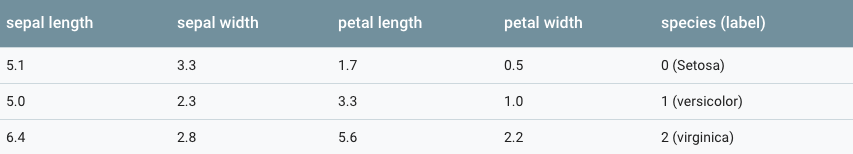
\includegraphics[width=\textwidth]{images/table}
  \caption{Data representation used for modeling (taken from~\cite{tensor18})}
  \label{fig:object-rep}
\end{figure}

\ac{NN} models are constructed based on the layers of neurons, the number of layers is determined 
by the data available to characterized a particular element. 
For the flower classification model, we used four layers. The two outer layers correspond to the 
indispensable input and output layers, while the two additional layers remain hidden in the net. 
The specific structure of the net is defined using the \tensorcode{DNNClassifier}, shown in 
\fref{lst:nn-definition}.  
The definition of the classifier requires the specification of the model's feature columns, hidden layers, 
and the different types of elements to classify.

\begin{tensorflow}[
	label={lst:nn-definition},
	caption={Neural network definition}]
 #Net contains 2 hidden layers with 10 nodes each.
 classifier = tf.estimator.DNNClassifier(
    feature_columns=my_feature_columns,
    hidden_units=[10, 10],
 #The model must choose between 3 classes which represent each flower.
    n_classes=3)
\end{tensorflow}

Additionally, we define an input function, shown in \fref{lst:input-definition}, specifying the features of 
the objects to recognize (following the same declaration of features as the initial data representation).

\begin{tensorflow}[
	label={lst:input-definition},
	caption={Input definition}]
 #Input function definition
 def input_evaluation_set():
    features = {'SepalLength': np.array([6.7, 5.3, 4.4]),
                'SepalWidth':  np.array([3.4., 4.2, 3.1]),
                'PetalLength': np.array([5.6, 3.3, 4.8]),
                'PetalWidth':  np.array([2.2, 1.0, 2.8])}
    labels = np.array([3, 1])
    return features, labels
\end{tensorflow}

Each of the input values is used to estimate it classification with respect to the original data model. 
This classification is described as a proportion of similarity for each of the classifiers (\ie types of 
elements defining the classes) representing how much the data relates to each of the classifiers.

For example, in the described for the input information in \fref{lst:input-definition}, the similarity 
proportion, for each type of flower, is that shown hereafter
\begin{enumerate}
 \item 0.08 for Iris Setosa
 \item 0.02 for Iris Versicolor
 \item 0.90 for Iris Virginica
\end{enumerate}

Based on these proportion, the model estimates that the observed flower (from the data) can be 
classified as and Iris Virginica flower. 

Note that as for the first experiment, in this case it is also necessary to train the model for recognition. 
The training data process for \ac{NN} is similar to that explained in the previous section through  
estimators provided as part of the TensorFlow API. 


%%%%
\subsection{Experiment Analysis}

For both, the housing system and flower classification experiments, their corresponding \ac{ML} 
models are trained using estimators to make accurate predictions. In the case of the California 
housing system, where there is a large amount of data with multiple classifications, we observe that 
the supervised \ac{ML} model for linear regression is the most appropriate technique for recovering 
specific traits featured in the data. This is drawn from the fact that no previous outcome was 
determined for the features used in the model. 
Furthermore, notice that the majority of the effort in the development process of the model is on 
adjusting the hyperparameters, which shape the model.  

Based on these observations, and the characteristic definitions of the model, we conclude that, 
indeed, linear regression models are adequate for predictions of large amounts of data. Additionally 
we remark that the linear regression model is an accessible technique for users starting to work with 
\ac{ML}.  

In the case of the flower classification experiment, the information was different as the features to 
examine were more constrained, the available information was smaller, and the prediction had to be 
classified among three types of flowers. Based on this, the linear regression model is no longer 
applicable, therefore the \tensorcode{DNNClassifier} was used to construct a \ac{NN}, enabling 
multi-class classification~\cite{tensor18}.
When using \ac{NN}, the complexity of the model's input reflects the shape of the network (taking into 
account how many layers are needed). Note that the model inherently provides a proportion of 
accuracy (\ie probability in the prediction) to classifying data. As a consequence, the model's 
precision improves over time. 

Finally, we remark that practitioners using \ac{ML} for a particular project, should only be concerned 
with the high-level API, providing out-of-the-box estimators appropriate to the specific \ac{ML} 
technique to use.


\endinput

